% Question 1
\question

\listbeginx	% start 1st level question
	\item \label{chemical} What chemical reactions you expect to see at these electrodes? 
	
	\translation{Apakah tindak balas kimia yang anda jangka dapat dilihat pada kedua –dua elektrod} 
	
	\qmarks{4}	% define marks
	
	\item A pair of biopotential electrodes is implanted in an animal to measure the electrocardiogram.
	
	\translation{Sepasang elektrod biopotensi diimplan ke dalam haiwan untuk mengukur elektrokardiogram.}

	\listbegin	% start 2nd level question
		\item Based on \ref{chemical}, explain what will happen if the electrodes were shorted together. Explain what will happen if the electrodes were shorted together. 
		
		\translation{Terangkan apakah yang akan berlaku apabila kedua – kedua elektrod disambung?. Terangkan apakah yang akan berlaku apabila kedua – kedua elektrod disambung?} 
		
		\qmarks{2} % define marks
	\listclose % close 2nd level question
	
	\item Explain what will happen if the capacitor in \cref{fig:meshcircuit} were shorted. 
	
	\translation{Terangkan apakah yang akan berlaku apabila kedua – kedua elektrod disambung?} 
	
	\qmarks{3} % define marks
		
	\begin{figure}[H] % H means, to put figure here after the code
		\centering
%		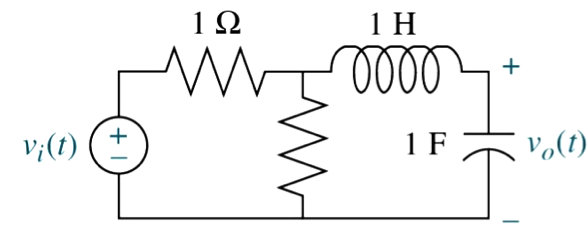
\includegraphics[width=0.5\textwidth]{testfig}
		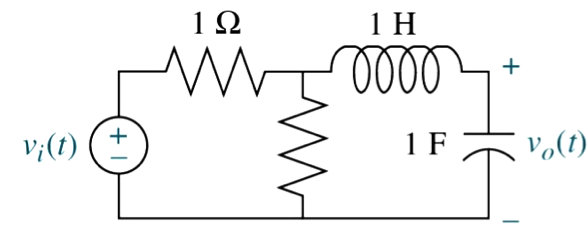
\includegraphics{testfig}
		\caption{\rajah}
		\label{fig:meshcircuit}
	\end{figure}

	% Table generated by Excel2LaTeX from sheet 'Sheet1'
	\begin{table}[H]
		\centering
		\caption{\jadual}
		\begin{tabular}{cc}
			\toprule
			\multicolumn{1}{l}{\textbf{Frequency}} & \multicolumn{1}{l}{\textbf{Impedance (Magnitude) ($\Omega$)}} \\
			\midrule
			5 Hz  & 20,000 \\
			10 Hz & 19,998 \\
			\vdots     & \vdots \\
			40 kHz & 602 \\
			50 kHz & 600 \\
			100 kHz & 600 \\
			\bottomrule
		\end{tabular}%
		\label{table:freqmag}%
	\end{table}%
\listclose % close 1st level question

